\section{Understanding the data and how its stored}
The data stored in these databases include filenames, access and creation dates, file attributes, and extended attributes. Depending on which table is viewed and what view is selected, there are currently 59 attributes(columns) per entry(row). Some of these attributes may be empty. More may be added in the future. \\
\\
Below are the most commonly used tables and views. 

\begin{figure} [h]
\centering
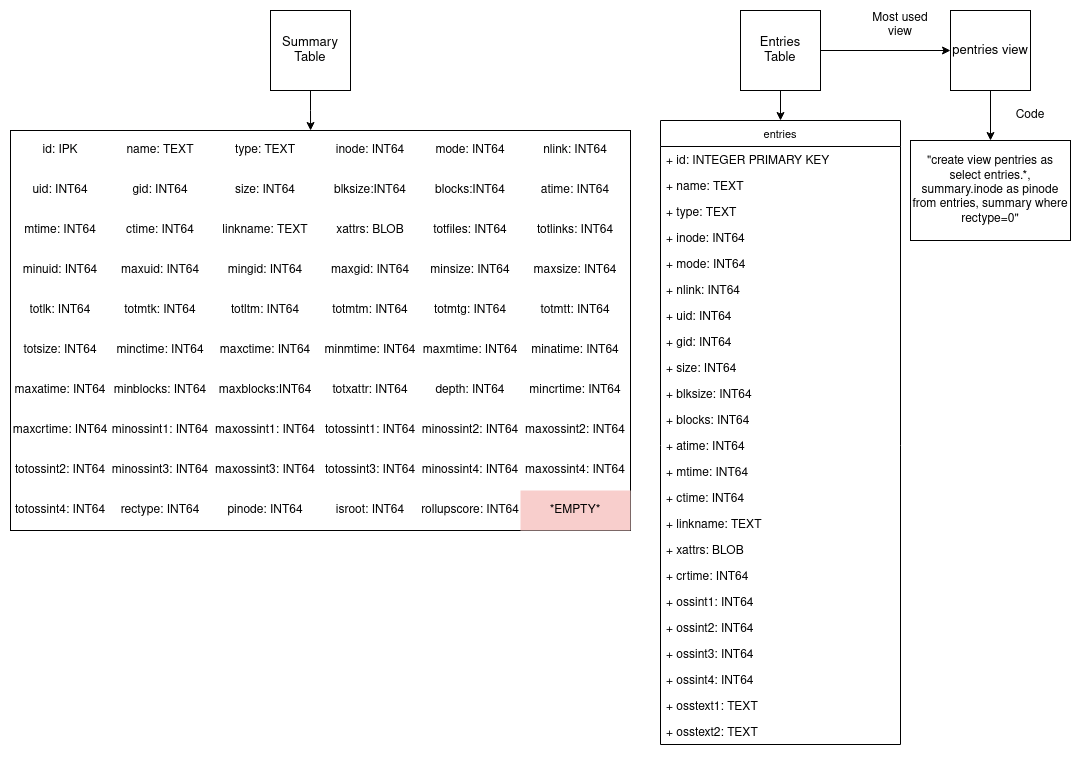
\includegraphics[width=1.0\textwidth]{images/Database_Schemas.png}
\caption{\label{fig:Database Schema}Database schema}
\end{figure}

\subsection{Why pentries is the most commonly used}
\begin{itemize}
  \item Provides parent inode as a query-able variable to the entries table
  \item Exists solely because parent inodes are not stored
  \item Parent inode is calculated/looked up so that parent inodes are never stored with child records.
\end{itemize}